
\documentclass[a4paper, 12p]{paper} 
\usepackage[margin=2.5cm]{geometry}
\usepackage{amsmath}
\usepackage{graphicx}
\usepackage{lipsum}
\usepackage{xcolor}
\usepackage{booktabs}
\usepackage{float}
\usepackage{subfigure}
\usepackage{titling}
\usepackage{kotex}
\usepackage{gensymb}
\usepackage{minted}
\usepackage{threeparttable}

\def\code#1{\texttt{#1}}
\sectionfont{\large\sf\bfseries\color{black!70!blue}}
\date{\vspace{-5ex}}
\renewcommand{\familydefault}{\sfdefault}
\renewcommand{\baselinestretch}{1.3} 

\pretitle{\centering\LARGE\bfseries}
\posttitle{\par}
\preauthor{\begin{flushright}\large}
\postauthor{\end{flushright}}

\title{Restoration of Gray Images}
\author{전자공학과 20161453 김규래}

\begin{document} 
\maketitle\hrule{}\bigskip

\section{Overview}
이번 과제의 목적은 Image noise filtering 과 Image reconstruction 을 구현함으로서 그 특징을 확인하는 것이다. 

\subsection{Padding}
모든 경우에 border extension padding 을 사용하였다.

\subsection{External Dependencies}
외부 라이브러리로는 OpenCV\footnote{https://opencv.org/} 를 사용하였다. OpenCV 에서는 다양한 영상처리 관련 루틴들을 제공하고 있으나, 본 과제에서는 \code{cv::imshow()} 와 \code{cv::imread()}, \code{cv::imwrite()}, \code{cv::dft()}, \code{cv::idft()}, \code{cv::calcHist()} 와 같은 기본적인 함수들만 사용하였으며 나머지는 전부 구현하였다.

\subsection{Installation}
시스템에 OpenCV 가 표준 경로에 설치돼있을 경우 CMake 에서 자동으로 인식을 할 것이다. 별도의 경로에 설치돼 있을 경우 \code{OpenCV\_ROOT\_DIR} 변수를 CMake 에 플래그로 넘김으로써 경로를 알려줄 수 있다. Blaze 의 경우에는 함께 첨부돼 있기 때문에 별도의 작업이 필요하지 않다. 다음과 같이 입력하면 빌드를 할 수 있다. 

\begin{align*}
  & \code{mkdir build \&\& cd build} \\
  & \code{cmake -G ``Unix Makefiles'' ..} \\
  & \code{make}
\end{align*}

\section{구현1}
구현1 에서는 uniform distribution, gaussian distribution, point mass 를 따르는 노이즈를 영상에 가한 다음, 그 분포를 히스토그램을 통해서 확인한다. 구현에서는 32비트 \textit{Mersenne-twister}\footnote{Matsumoto, Makoto, and Takuji Nishimura. "Mersenne twister: a 623-dimensionally equidistributed uniform pseudo-random number generator." ACM Transactions on Modeling and Computer Simulation (TOMACS) 8.1 (1998): 3-30.} 난수 발생기를 사용하였다.

\begin{figure}[H]
\centering
\subfigure[Original]{

\includegraphics[scale=0.53]{../data/Pattern.png}
}
\subfigure[Uniform, 23.97 dB]{
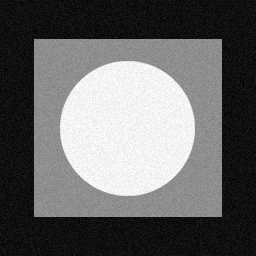
\includegraphics[scale=0.4]{../data/uniform.png}
}
\subfigure[Gaussian, 19.69 dB]{
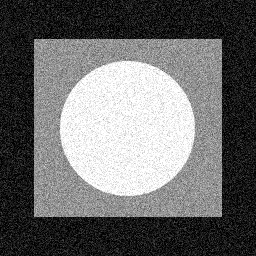
\includegraphics[scale=0.4]{../data/gaussian.png}
}
\subfigure[Salt and Pepper, 10.92 dB]{
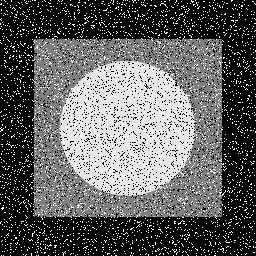
\includegraphics[scale=0.4]{../data/saltpepper.png}
}
\caption{다양한 분포의 노이즈들을 영상에 더했을 때의 결과물. dB 로 표기된 숫자는 \textit{Signal-to-Noise Ratio} (PSNR) 이다. }\label{fig:noise}
\end{figure}

원본 영상이 $x$ 이고, 노이즈로 손상된 영상이 $y$ 며, 덧셈 노이즈를~\eqref{eq:additive} 와 같이 가정할 때, \textit{Uniform}~\eqref{eq:uniform}, \textit{Gaussian}~\eqref{eq:normal}, 그리고 \textit{salt and pepper}~\eqref{eq:saltpepper} 를 따르는 세 종류의 노이즈를 영상에 첨가한 모습을 Fig.\ref{fig:noise} 에서 볼 수 있다.  각 사진의 캡션에 표기된 숫자는 \textit{Signal-to-Noise Ratio} (PSNR) 를 의미한다. 노이즈를 더하면서 영상의 PSNR 이 낮아지는 것을 알 수 있다. 특히 salt and pepper noise 의 경우 손상으로 발생하는 값들이 극단적이라서 PSNR 이 특히 좋지 못하다.

\begin{align}
  y &= x + \epsilon \label{eq:additive} \\
  \epsilon &\sim Uniform(5, 25) \label{eq:uniform} \\
  \epsilon &\sim \mathcal{N}(\mu=20, \sigma=20) \label{eq:normal} \\
  p(\epsilon = 0) &= 0.1, \;\;\; p(\epsilon = 255) = 0.1 \label{eq:saltpepper}
\end{align}

\begin{figure}[H]
\centering
\subfigure[Original]{
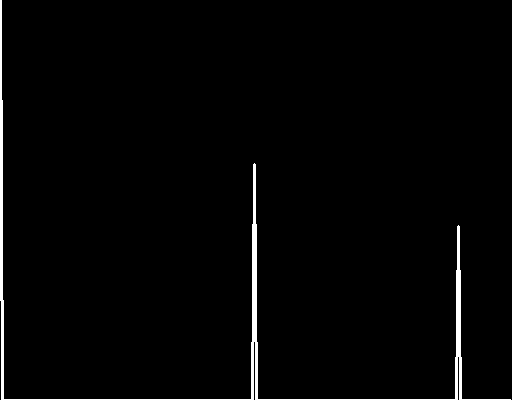
\includegraphics[scale=0.2]{../data/original_hist.png}
}
\subfigure[Uniform]{
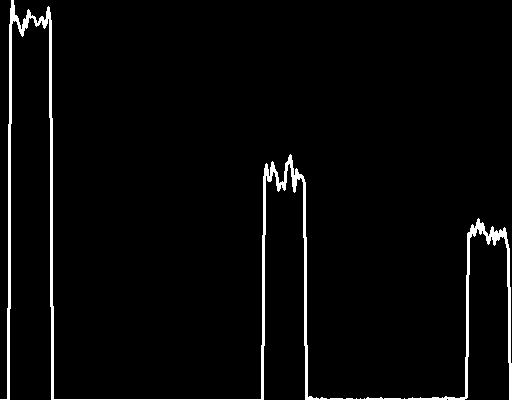
\includegraphics[scale=0.2]{../data/uniform_hist.png}
}
\subfigure[Gaussian]{
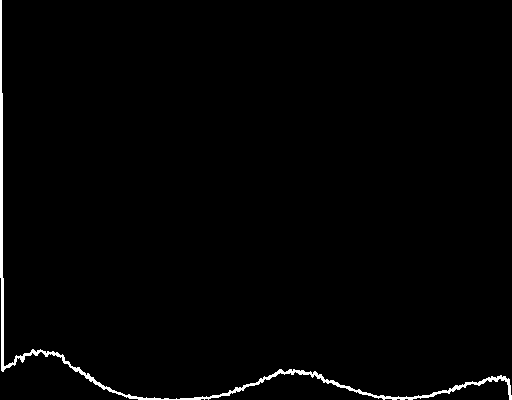
\includegraphics[scale=0.2]{../data/gaussian_hist.png}
}
\subfigure[Salt and Pepper]{
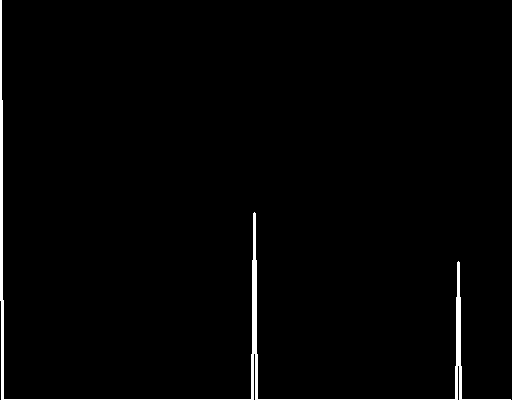
\includegraphics[scale=0.2]{../data/saltpepper_hist.png}
}
\caption{다양한 분포의 노이즈들을 영상에 더했을 때의 픽셀 히스토그램.}\label{fig:hist}
\end{figure}

이 때 노이즈를 첨가한 영상들의 히스토그램은 Fig.~\ref{fig:hist} 와 같다. 이로부터 각 노이즈 분포들의 특징을 확인할 수 있다. Uniform noise 의 경우 평탄한 형태의 노이즈가 생기며, gaussian 은 원래의 intensity 주변에 gaussian smoothing 비슷한 효과를 보인다. 마지막으로 salt and pepper noise 의 경우 극단적인 값들의 크기가 상대적으로 커지는 것을 볼 수 있다.

\section{구현2}
이번 구현에서는 noise filter 들을 이용해서 salt and pepper noise 를 filtering 한다. 주어진 영상들 중에 어떤 것을 사용핸야된다는 특별한 지시가 없어 \code{Ckt\_board\_salt\&pepper\_0.3.tif} 를 사용하였다. Median filter, contraharmonic mean, 그리고 adaptive median 총 세 종류의 필터들을 구현하였다.

\subsection{Median filter}
첫째로, median filter 를 구현한 코드는 아래와 같다. 먼저 지정된 크기의 patch  내의 픽셀들을 \code{buffer} 에 저장한 다음, median 을 계산한 후 patch 의 중심이 되는 픽셀의 값을 median 으로 대체한다.

  \begin{minted}
    [frame=lines,
      framesep=2mm,
      baselinestretch=0.5]{cpp}
#pragma omp parallel for schedule(static) collapse(2)
    for(size_t i = 0; i < m; ++i) {
        for(size_t j = 0; j < n; ++j) {
            auto buffer = std::vector<uint8_t>(window_elems);
            /* Load patch to buffer */
            for(size_t u = 0; u < window_size; ++u) {
                for(size_t v = 0; v < window_size; ++v) {
                    buffer[u + v * window_size] =
                        fetch_pad(src, i + u, j + v, m, n, offset_m, offset_n);
                }
            }
            /* Compute median */
            auto pix = median<uint8_t>(buffer.begin(), buffer.end(), window_elems);

            /* Store median of patch to image */
            dest.at<uint8_t>(i, j) = pix;
        }
    }
  \end{minted}

\subsection{Contraharmonic Mean filter}
Contraharmnic filter 의 경우에는 동작이 median filter 와 유사하나, patch 중심 픽셀을 median 으로 대체하는 대신에 patch 의 각 픽셀들을 $Q$ 번째 power 를 구하고 전부 더한 다음 $Q+1$ 번째 power 들의 합으로 나눈 값을 사용한다. 구현한 코드는 아래와 같다.

  \begin{minted}
    [frame=lines,
      framesep=2mm,
      baselinestretch=0.5]{cpp}
#pragma omp parallel for schedule(static) collapse(2)
    for(size_t i = 0; i < m; ++i) {
        for(size_t j = 0; j < n; ++j) {
            /* Load patch to buffer */
            auto buffer = std::vector<uint8_t>(window_elems);
            for(size_t u = 0; u < window_size; ++u) {
                for(size_t v = 0; v < window_size; ++v) {
                    buffer[u + v * window_size] =
                        fetch_pad(src, i + u, j + v, m, n, offset_m, offset_n);
                }
            }

            double num = 0;
            double den = 0;
            /* Compute numerator and denominator */
            for(size_t i = 0; i < window_elems; ++i)
            {
                auto prod = pow(static_cast<double>(buffer[i]), Q);
                den += prod;
                num += prod * buffer[i];
            }

            /* Store computed value */
            dest.at<uint8_t>(i, j) = cv::saturate_cast<uint8_t>(num / den);
        }
    }
  \end{minted}

\subsection{Adaptive Median filter}
Adaptive median filter 의 경우에는 median filter 의 뛰어난 필터링 효과를 더 극대화하기 위해, image patch 의 크기를 patch 의 통계적인 수치들을 이용해서 adaptive 하게 결정하는 알고리즘이다. Patch 의 median 값이 최대값이나 최소값과 같을 경우, patch 가 충분한 정보를 담지 못하고 있다고 판단하고 patch 의 크기를 키운다. 코드는 아래와 같다. $S\_max$ 파라미터의 경우 16 으로 설정하였다.

  \begin{minted}
    [frame=lines,
      framesep=2mm,
      baselinestretch=0.5]{cpp}
#pragma omp parallel for schedule(static) collapse(2)
    for(size_t i = 0; i < m; ++i) {
        for(size_t j = 0; j < n; ++j) {
            auto window_size = initial_window_size;
            uint8_t pix      = 0;
            auto zxy         = src.at<uint8_t>(i, j);
            while(true)
            {
                /* Load patch to buffer */
                size_t offset       = floor(window_size / 2.0);
                size_t window_elems = window_size * window_size;
                auto buffer = std::vector<uint8_t>(window_elems);
                for(size_t u = 0; u < window_size; ++u) {
                    for(size_t v = 0; v < window_size; ++v) {
                        buffer[u + v * window_size] =
                            fetch_pad(src, i + u, j + v, m, n, offset, offset);
                    }
                }

                /* Compute patch statistics */
                auto median_iter = buffer.begin() + floor(window_elems / 2.0);
                std::nth_element(buffer.begin(), median_iter, buffer.end());
                auto zmed = *median_iter;
                std::nth_element(buffer.begin(), buffer.begin(), median_iter);
                auto zmin = *buffer.begin();
                std::nth_element(median_iter, buffer.begin() + window_elems - 1, buffer.end());
                auto zmax = *(buffer.begin() + window_elems - 1);

                /* Termination condition */
                if(zmin < zmed && zmed < zmax)
                {
                    pix = zmin < zxy && zxy < zmax ? zxy : zmed;
                    break;
                }
                window_size += 2;
                if(window_size >= window_max)
                {
                    pix = zmed;
                    break;
                }
            }
            dest.at<uint8_t>(i, j) = pix;
        }
    }
  \end{minted}

  Adaptive median filter 의 경우 image patch 의 중간값, 최소값, 쵀대값을 모두 계산하여야 하는데, 이 값들을 전부 계산하는 효율적인 방법에는 두가지가 있다. 첫 째는 patch 의 값들을 전부 한번에 정렬한 다음에 원하는 값들을 바로 가져가는 것이고, 두 번째는 \textit{nth element} 정렬 방법을 통해서 부분 정렬을 3번 하는 것이다. nth element 를 통한 부분 정렬을 선택하는 경우, 먼저 median 을 계산하고, median 을 중심으로 앞쪽의 값들을 다시 한번 정렬해서 최솟값을 구하고, 뒤쪽의 값들을 또 다시 정렬해서 최대값을 구할 수 있다. 전체를 정렬은 복잡도가 일반적으로 $O(N \log N)$ 이고, nth element 정렬은 $O(N)$ 이기 때문에 이론적으로는 nth element 를 3번 하는 것이 더 좋은 성능을 얻는다. 이를 확실히 비교하기 위해서 두 가지를 모두 구현한 다음 성능을 비교해보았다.

\begin{figure}[H]
\centering
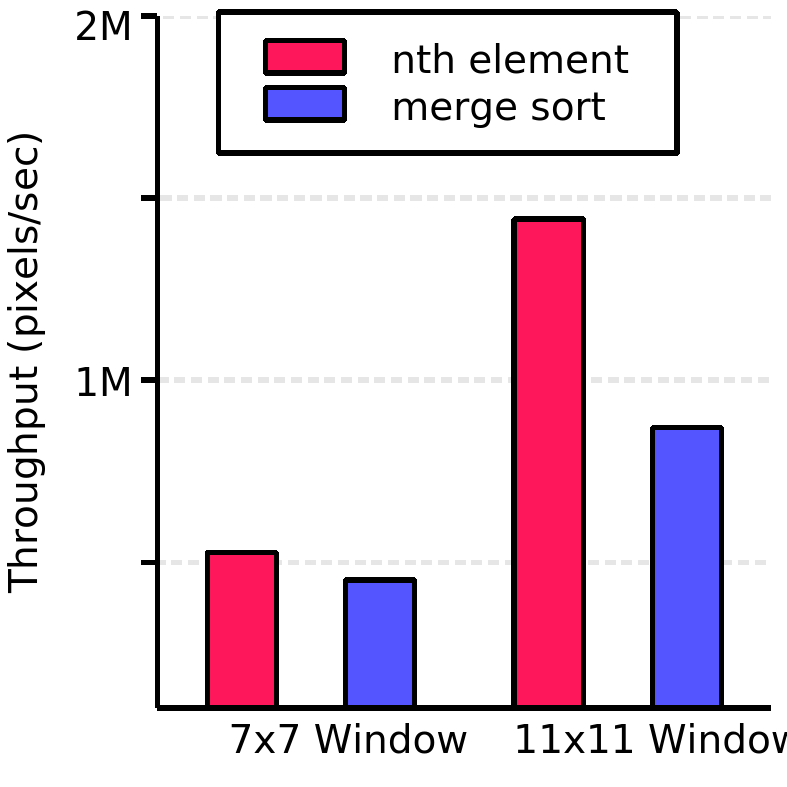
\includegraphics[scale=0.5]{../data/adapt_perf.png}\label{fig:perf}
\end{figure}

비교 결과는 Fig.~\ref{fig:perf} 에서 볼 수 있다. $n$th element 를 사용한 경우가 확실히 성능이 더 좋으며, 이는 기본 patch 크기가 커질수록 더 명확해진다. 


\subsection{결과분석}
이전 섹션들에서 구현한 필터들을 주어진 \code{Ckpt\_board.tif} 에 노이즈가 더해진 영상들에 적용을 해보았다. 어떠한 영상을 사용할지에 관해 특별한 언급이 없어 손상이 큰 편인 $p=0.3$ 의 Salt and pepper 노이즈가 더해진 영상을 사용하였다.

\begin{figure}[H]
\centering
\subfigure[Corrupted, 10.12 dB]{
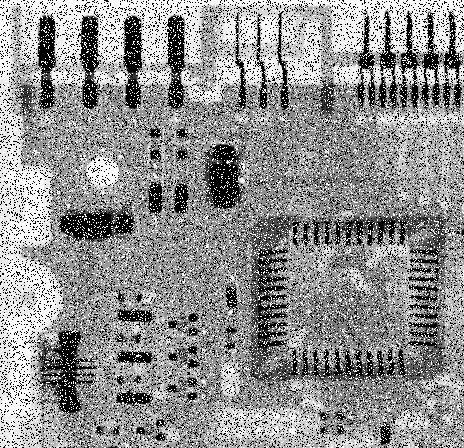
\includegraphics[scale=0.29]{../data/Ckt_board_salt&pepper_0p3.png}
}
\subfigure[Median $3 \times 3$, 21.59 dB]{
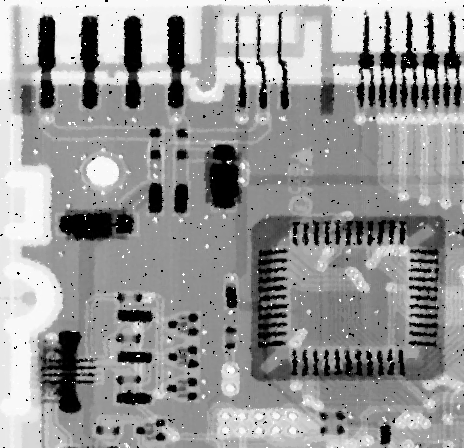
\includegraphics[scale=0.22]{../data/median_3.png}
}
\subfigure[Median $5 \times 5$, 23.26 dB]{
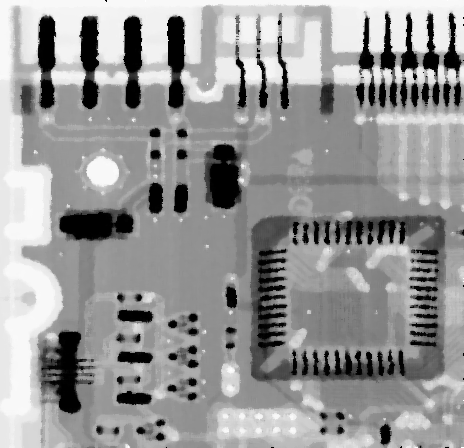
\includegraphics[scale=0.22]{../data/median_5.png}
}
\subfigure[Contra. $Q=1.5$, 10.08 dB]{
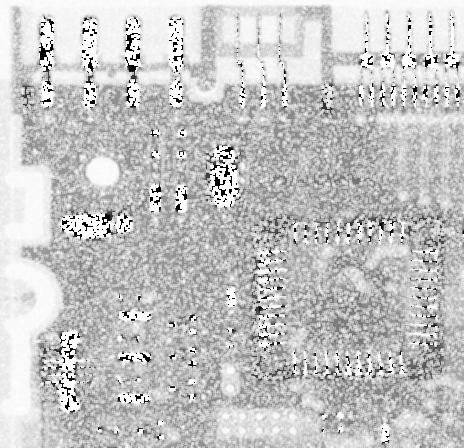
\includegraphics[scale=0.22]{../data/contraharmonic_1p5.png}
}
\subfigure[Contra. $Q=0$, 17.14 dB]{
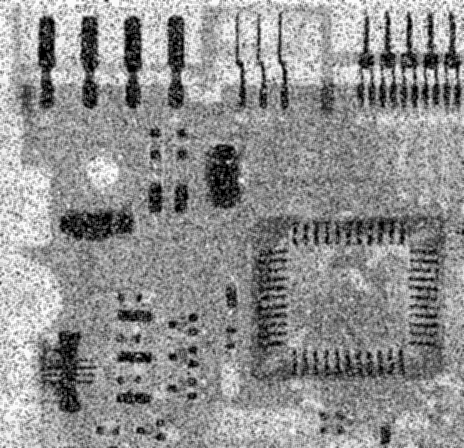
\includegraphics[scale=0.22]{../data/contraharmonic_0.png}
}
\subfigure[Contra. $Q=-1.5$, 4.93 dB]{
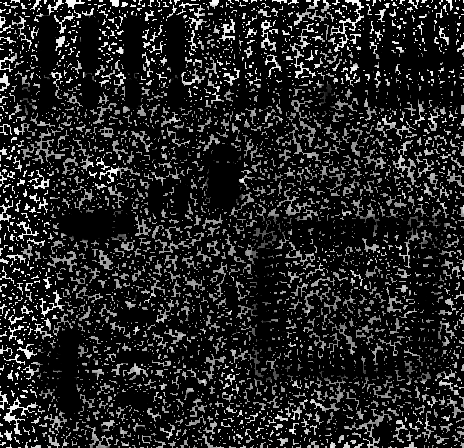
\includegraphics[scale=0.22]{../data/contraharmonic_m1p5.png}
}
\subfigure[Adaptive $7 \times 7$, 24.20 dB]{
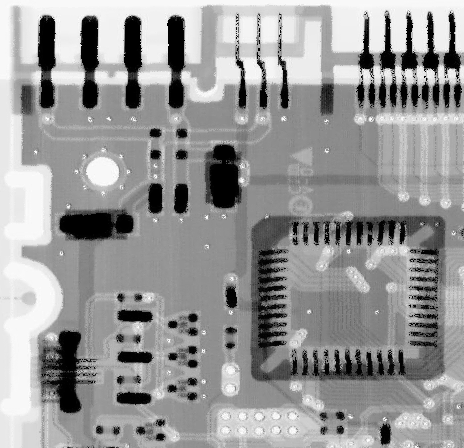
\includegraphics[scale=0.22]{../data/apaptive_7.png}
}
\subfigure[Adaptive $11 \times 11$, 20.58 dB]{
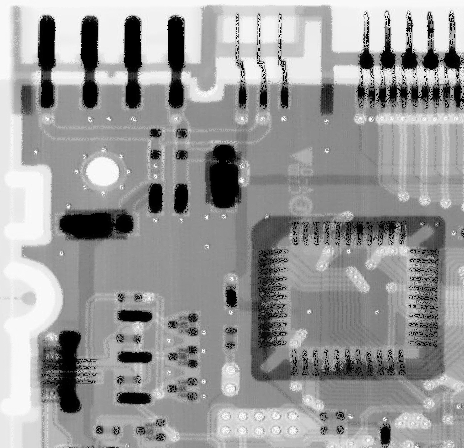
\includegraphics[scale=0.22]{../data/adaptive_11.png}
}
\caption{Noise filter 들을 적용하여 영상을 복원해낸 결과물.}\label{fig:filtered}
\end{figure}

\textit{Median filter}, \textit{Contraharmonic Mean filter} (Contra.), \textit{Adaptive Median filter}, 총 세종의 필터를 다양한 파라미터 세팅에서 적용해본 결과를~Fig.\ref{fig:filtered} 에서 볼 수 있다. Median filter 와 Adaptive median filter 는 복원 효과가 굉장히 좋다는 것을 확인할 수 있다. 특히 $7x7$ Adaptive median filter 는 가장 높은 PSNR 을 보였다.

Contra. filter의 경우에는 반대로 원본 영상에 비해 PSNR 이 감소하는 것으로 나타났는데, 이는 사용한 영상의 노이즈 레벨이 워낙 컸기 때문으로 보인다. 노이즈 레벨이 더 낮은 영상을 사용할 경우 Contra. filter 도 어느 정도의 노이즈 제거 효과를 보였다. 사용한 영상에 한해서 분석을 해보면, $Q=1.5$ 일 때 밝은 부분에서 pepper noise 제거 효과가 확실히 나타나고, $Q=-1.5$ 일 때는 어두운 부분에서 확실한 salt noise 제거 효과가 보인다. $Q=0$ 일 때는 mean filter 와 동일한데 예상할 수 있듯이 영상이 blur 되는 효과만 나타났다. Salt and pepper noise 의 극단적인 수치들로 인해서 mean filter 는 효과가 크지 않다는 것을 고려할 때 예상할 수 있는 결과이다.

\begin{figure}[H]
\centering
\subfigure[Corrupted, 10.12 dB]{
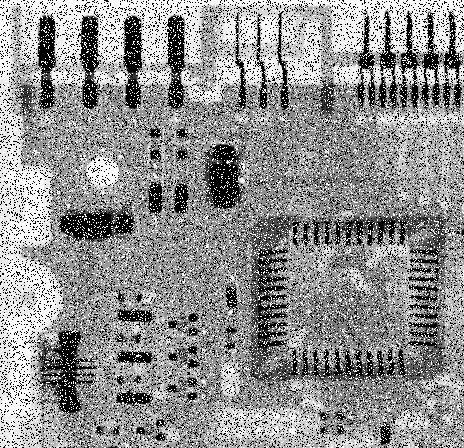
\includegraphics[scale=0.23]{../data/Ckt_board_salt&pepper_0p3.png}
}
\subfigure[1 time, 23.26 dB]{
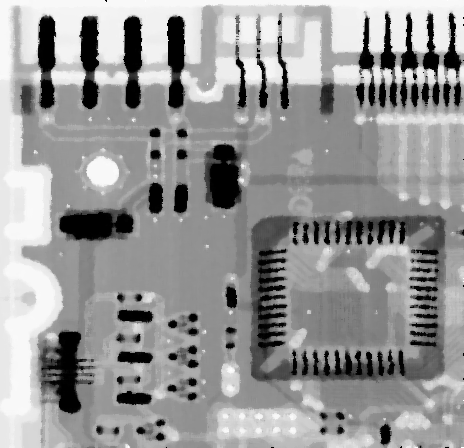
\includegraphics[scale=0.17]{../data/median_5.png}
}
\subfigure[2 times, 22.73 dB]{
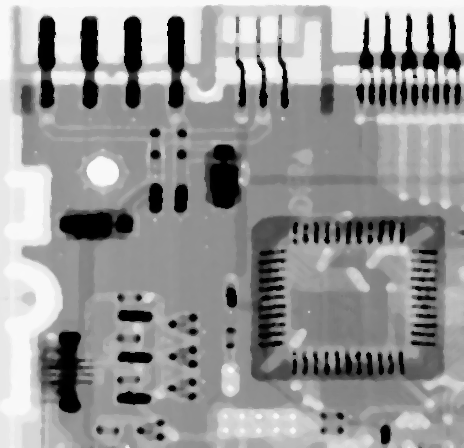
\includegraphics[scale=0.17]{../data/median_twice.png}
}
\subfigure[3 times, 21.86 dB]{
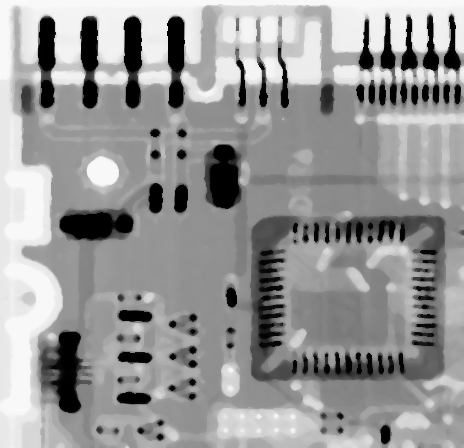
\includegraphics[scale=0.17]{../data/median_third.png}
}
\subfigure[4 times, 21.17 dB]{
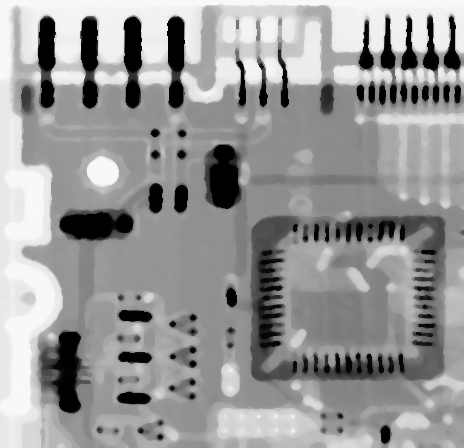
\includegraphics[scale=0.17]{../data/median_fourth.png}
}
\caption{$5 \times 5$ Median filter 를 어려번 적용했을 때 영상의 변화}\label{fig:median_many}
\end{figure}

\noindent\textbf{검토사항:} $5 \times 5$ Median filter 를 여러번 영상에 적용했을 때 변화하는 모습을 \ref{fig:median_many} 에서 볼 수 있다. Median filter 여러 횟수 적용할 수록 가시적인 노이즈가 줄어드나, 영상의 디테일 줄어들면서 PSNR 이 안 좋아지는 것을 알 수 있다. Median filter 도 다른 필터들과 비슷하게 low-pass 의 일종으로 볼 수 있는데, 지속적으로 적용할수록 high frequency 성분이 감소하고 영상의 원본 신호 대역까지 제거되면서 손상이 발생하는 것으로 생각할 수 있다. 따라서 Median filter 를 여러번 적용하는 것은 디테일을 포기하고 노이즈를 완벽하게 제거해야되는 상황이 아닌 이상 피하는 것이 좋다.

\section{구현3}
\subsection{개요}

이번 구현에서는 convolution 으로 표현되는 영상의 degradation 을 inverse filtering (deconvolution) 과 weiner filtering 을 이용해서 복원하는 것이다. 영상 f 에 대해서 degradation 이 어떠한 degradation model h 에 대해서~\eqref{eq:degrad} 와 같이 표현이 될 때, frequency domain 에서는~\eqref{eq:cplx_degrad} 으로 표현이 된다. 여기서 n 과 N 은 어떠한 random noise 를 의미한다.

\begin{align}
  g(x, y) &= h(x, y) * f(x,  y) + n(x, y) \label{eq:degrad} \\
  G(u, v) &= H(u, v) F(u, v) + N(u, v) \label{eq:cplx_degrad}
\end{align}

이에 대해서 이번 구현에서는 두 가지 필터를 사용하는데, 각각 inverse filter~\eqref{eq:inv} 와 Weiner filter~\eqref{eq:weiner} 이다.

\begin{align}
  \hat{F}(u, v) &=
  \begin{cases} 
    G(u, v)\frac{1}{H(u, v)}  & if \;\; u^2 + v^2 \leq r^2 \\
    G(u, v)                   & if \;\; u^2 + v^2  > r^2
  \end{cases} \label{eq:inv} \\
  \hat{F}(u, v) &= G(u, v)\frac{1}{H(u, v)}\frac{|H(u, v)|^2}{|H(u, v)|^2 + \frac{S_n(u, v)}{S_s(u, v)}} \label{eq:weiner}
\end{align}

주어진 degradation model 은~\eqref{eq:degrad} 와 같은데, $H \in \mathcal{R}$ 이기 때문에 Weiner filter 는 \eqref{eq:weiner} 와 같은 형태로 간단하게 계산이 가능하다. 이 때 $S_n/S_s$ 은 노이즈 $N(u, v)$과 원래 신호 $F(u, v)$ 의 비율을 의미한다. 자세한 관련 얘기는 아래 검토사항에서 다루도록 하겠다.

\begin{align}
  H(u, v) = e^{-k {(u^2 + v^2)}^{5/6}} \label{eq:degrad} \\
  \hat{F}(u, v) = G(u, v)\frac{{H(u, v)}^2}{H(u, v)({H(u, v)}^2 + \frac{S_N(u, v)}{S_s(u, v)})} \label{eq:weiner}
  \
\end{align}
 
\subsection{구현}

위 공식들과 같이 두 종류의 필터들을 구현하였다. 문제는 inverse filtering 을 할 때는 필터링을 적용하는 범위의 radius $r$ 을 결정해야하는데, 여러가지 값을 실험해본 결과를 Table.~\ref{table:radius} 에 정리한 대로 시험해본 결과, $r^2 = 64$ 일 때가 괜찮은 평균 성능을 얻을 수 있었다.

\begin{table*}[ht]
  \centering
\begin{threeparttable}
  \caption{PSNR Relative to Filtering Radius}\label{table:radius}
\begin{tabular}{l | r r r r r }
 $\text{Radius}^2$ & 16    & 32    & \textbf{64}   & 128   & 256   \\ \hline
  \toprule
0.00025            & 25.73 & 25.74 & \textbf{25.84} & 26.69 & 32.16 \\ \hline
0.001              & 22.09 & 22.15 & \textbf{22.60} & 24.75 & 6.44  \\ \hline
0.0025             & 20.71 & 20.91 & \textbf{21.92} & 10.84 & 4.73  \\ \hline
\bottomrule
$\mu$              & 22.84 & 22.93 & \textbf{23.45} & 20.76 & 14.44 \\ \hline
\end{tabular}
\end{threeparttable}\\
\end{table*}

Weiner filter 에서 사용되는 파라미터 $K = \frac{S_n(u, v)}{S_s(u, v)}$ 의 경우, 이론적으로는 quantization noise 의 비율인 $1 / 255$ 로 설정하는 것이 적절하나, 실험 결과 $1/1000$ 정도가 더 좋은 성능을 얻어냈기에 그렇게 설정하였다.

\begin{figure}[H]
\centering
\subfigure[Inverse, $k=0.00025$]{
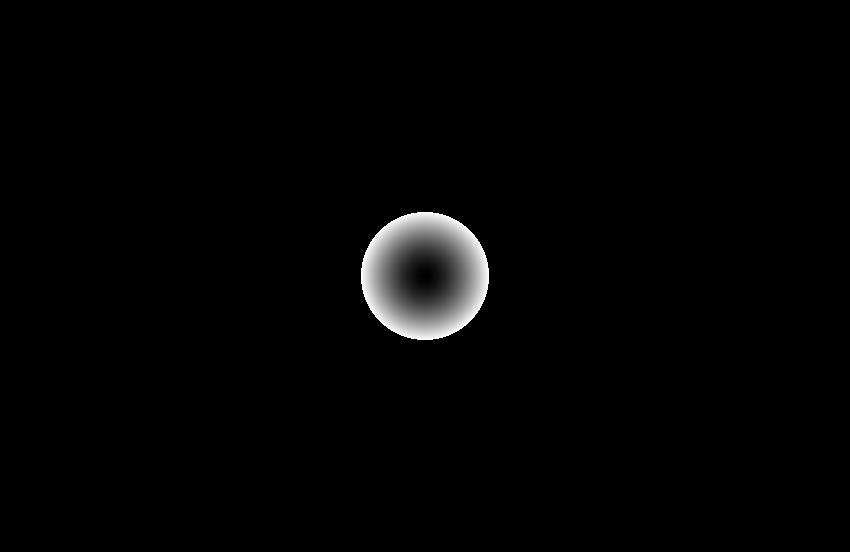
\includegraphics[scale=0.15]{../data/sogang_0p00025_sepc_undegrad.png}
}
\subfigure[Inverse, $k=0.001$]{
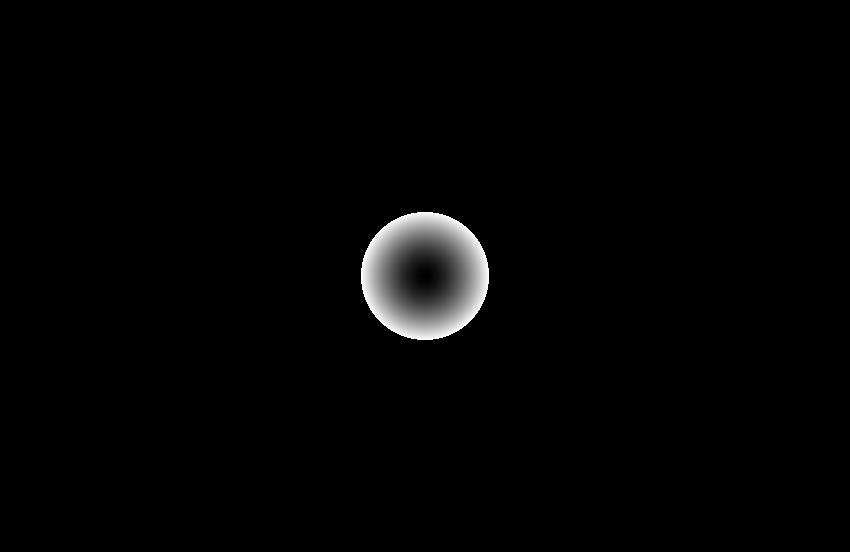
\includegraphics[scale=0.15]{../data/sogang_0p001_sepc_undegrad.png}
}
\subfigure[Inverse, $k=0.0025$]{
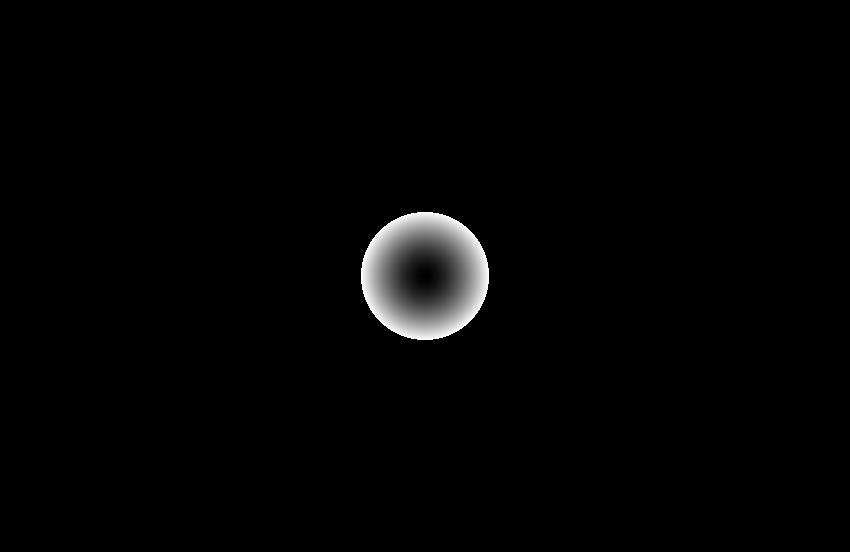
\includegraphics[scale=0.15]{../data/sogang_0p0025_sepc_undegrad.png}
}
\subfigure[Weiner, $k=0.00025$]{

\includegraphics[scale=0.15]{../data/sogang_wienerp00025_sepc_undegrad.png}
}
\subfigure[Weiner, $k=0.001$]{
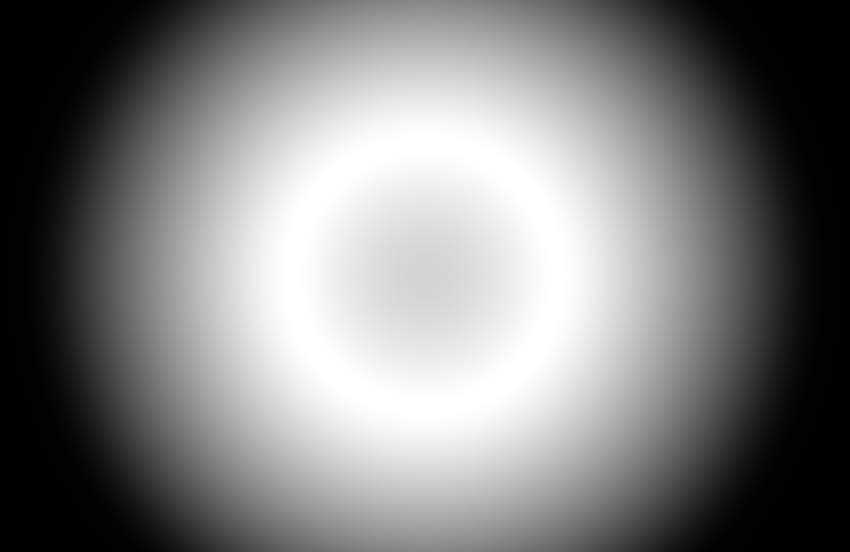
\includegraphics[scale=0.15]{../data/sogang_wienerp001_sepc_undegrad.png}
}
\subfigure[Weiner, $k=0.0025$]{
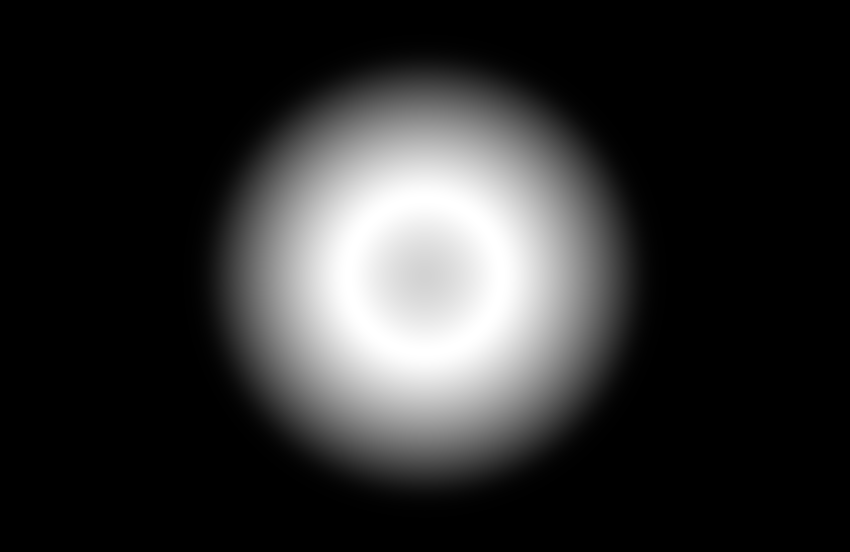
\includegraphics[scale=0.15]{../data/sogang_wienerp0025_sepc_undegrad.png}
}
\caption{복원에 사용되는 필터들의 frequency domain 스팩트럼.}\label{fig:degrad}
\end{figure}

두 종류의 복원 필터들을 서로 다른 $k$값에 대해서 생성한 스펙트럼을 Fig.\ref{fig:degrad} 에서 볼 수 있다. Inverse filter 들의 경우 적용되는 범위를 제한함으로 인해서 중앙을 기준으로 작은 범위에 대해서만 응답이 있다. Weiner filter 의 경우에는 자연적으로 응답 범위가 조절되는 것을 볼 수 있다.

\subsection{결과 분석}
주어진 영상 \code{Sogang.tif} 에 두가지 필터들을 각각 적용해보았다.

\begin{figure}[htbp]
\centering
\subfigure[Degraded, $k=0.00025$]{
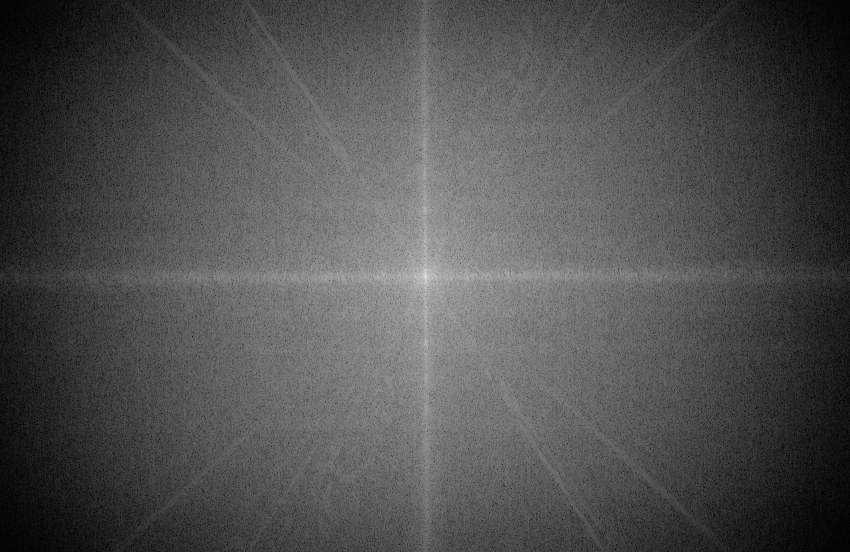
\includegraphics[scale=0.15]{../data/sogang_0p00025_spec_degraded.png}
}
\subfigure[Inverse, $k=0.00025$]{
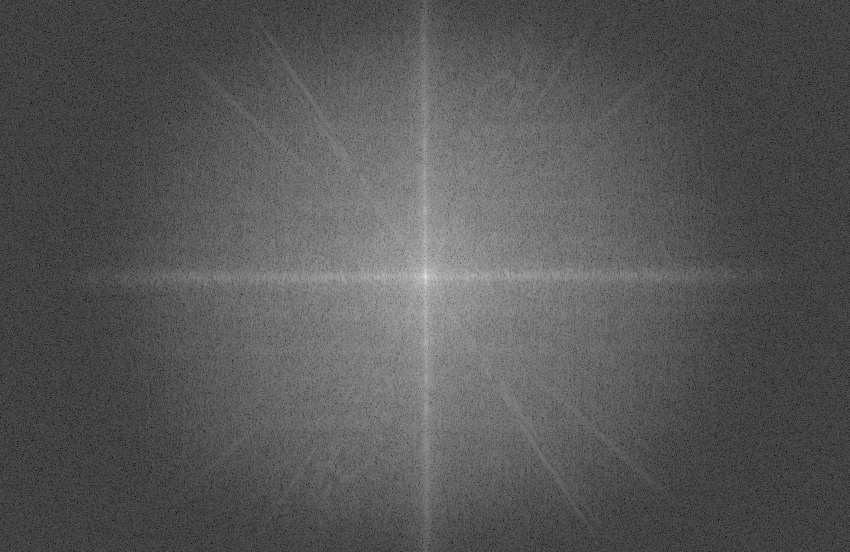
\includegraphics[scale=0.15]{../data/sogang_0p00025_spec_undegraded.png}
}
\subfigure[Weiner, $k=0.00025$]{
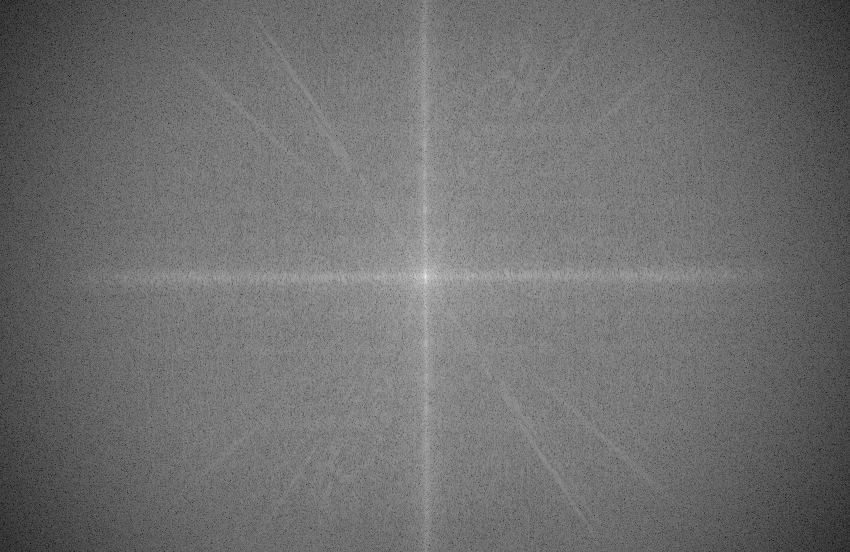
\includegraphics[scale=0.15]{../data/sogang_wienerp00025_spec_undegraded.png}
}
\subfigure[Degraded, $k=0.001$]{
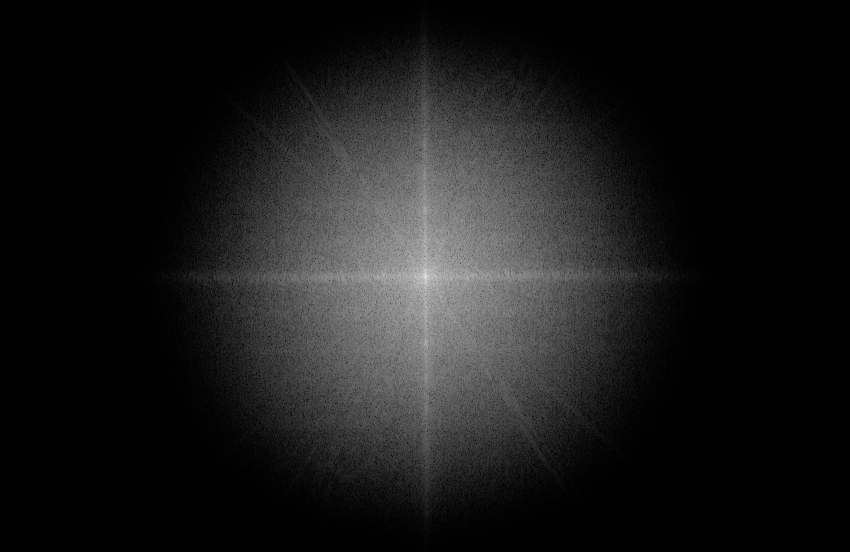
\includegraphics[scale=0.15]{../data/sogang_0p001_spec_degraded.png}
}
\subfigure[Inverse, $k=0.001$]{
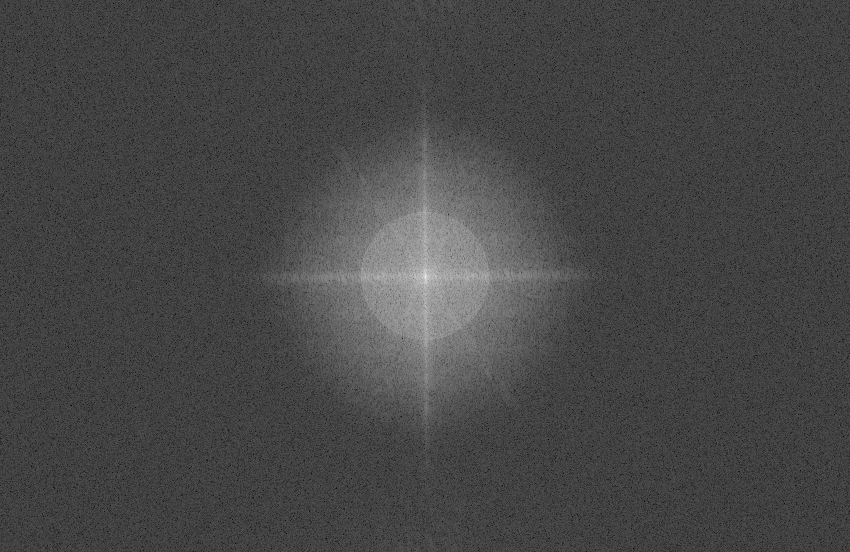
\includegraphics[scale=0.15]{../data/sogang_0p001_spec_undegraded.png}
}
\subfigure[Weiner, $k=0.001$]{
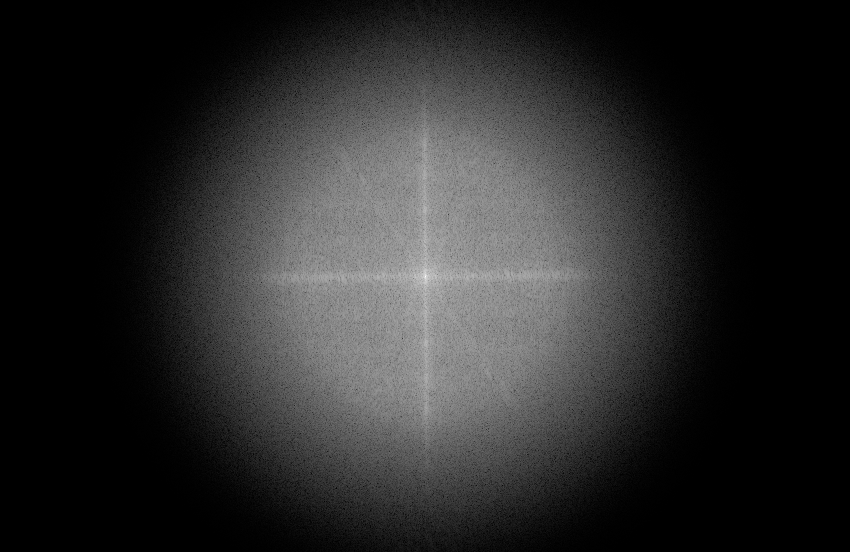
\includegraphics[scale=0.15]{../data/sogang_wienerp001_spec_undegraded.png}
}
\subfigure[Degraded, $k=0.0025$]{
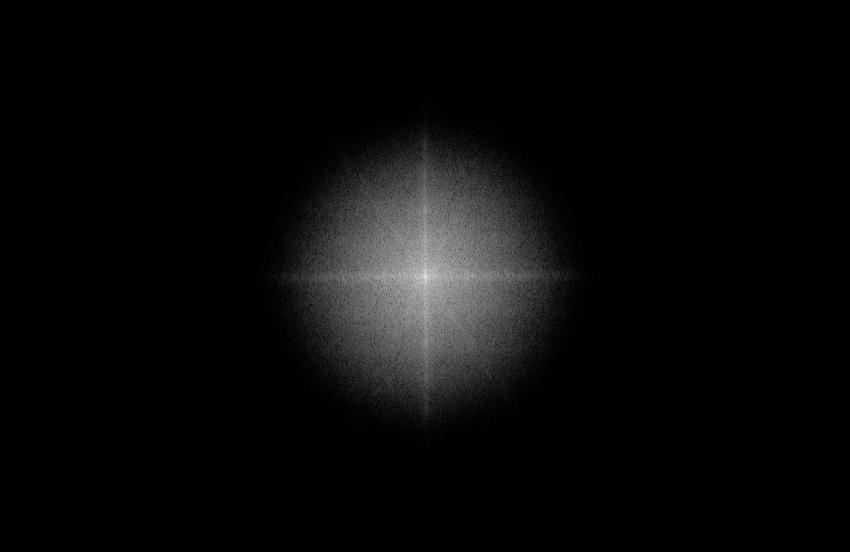
\includegraphics[scale=0.15]{../data/sogang_0p0025_spec_degraded.png}
}
\subfigure[Inverse, $k=0.0025$]{
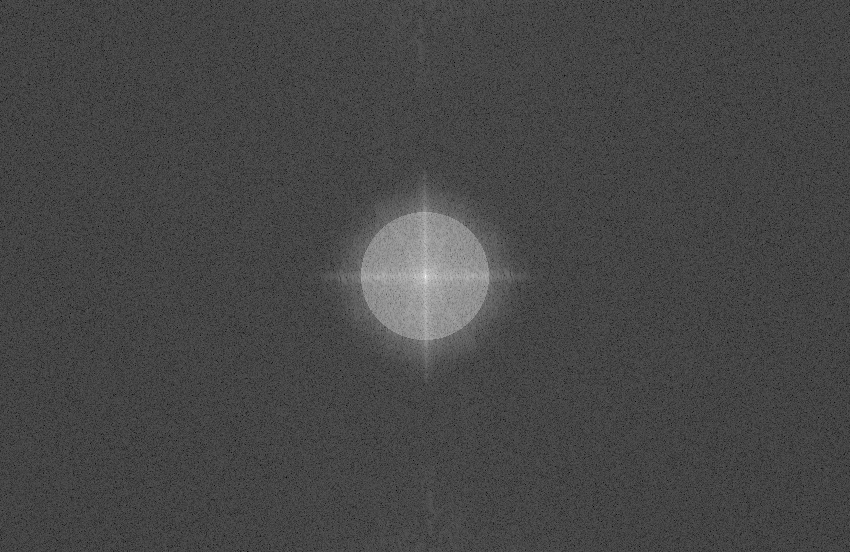
\includegraphics[scale=0.15]{../data/sogang_0p0025_spec_undegraded.png}
}
\subfigure[Weiner, $k=0.0025$]{
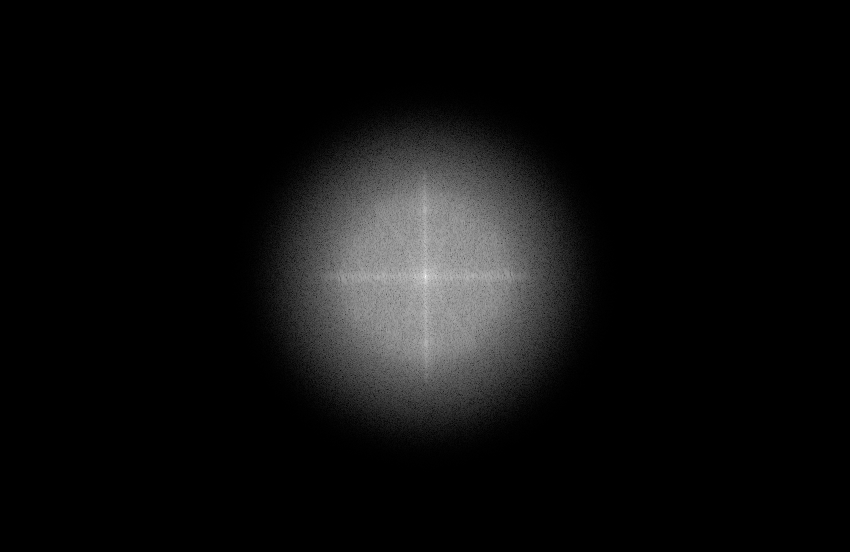
\includegraphics[scale=0.15]{../data/sogang_wienerp0025_spec_undegraded.png}
}
\caption{복원을 적용한 영상들의 frequency domain spectrum.}\label{fig:filter_spec}
\end{figure}

Fig.~\ref{fig:filter_spec} 을 보면 degradation 이 적용된 스팩트럼과, 복원이 적용된 스팩트럼을 비교해볼 수 있다. Degradation 이 적용된 스팩트럼은 고주파 성분이 손실된 것을 볼 수 있고, inverse filter 를 적용한 경우 복원 영역 내의 신호는 급격하게 커졌다. Weiner filter 를 적용한 경우 degradation 이 적용된 스팩트럼보다 스팩트럼이 조금 넓게 복원 되는 것을 볼 수 있다. 두 가지 경우 모두 주파수 전 영역이 아니라 저주파 대역 일부에서는 복원이 이뤄졌다. 이에 대한 이유는 아래 검토사항에서 다룬다.

\begin{figure}[tbp]
\centering
\subfigure[Degraded, $k=0.00025$, 25.72 dB]{
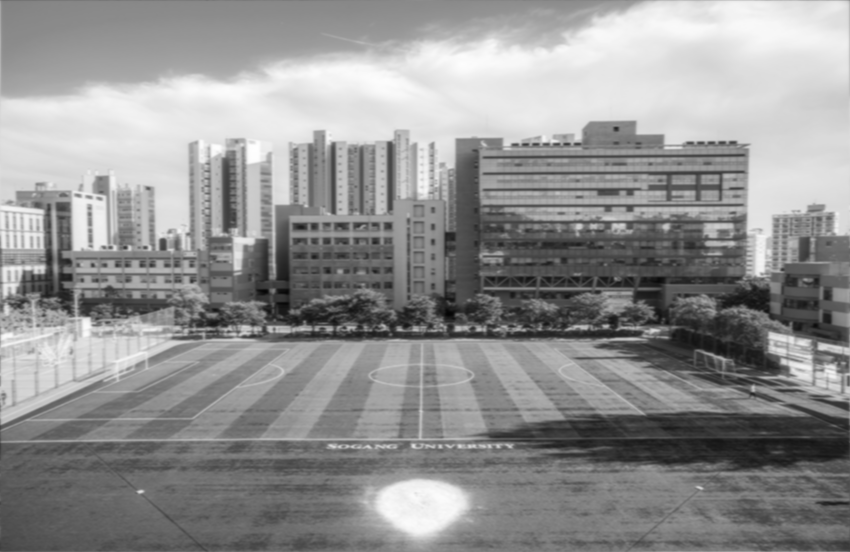
\includegraphics[scale=0.15]{../data/sogang_0p00025_degraded.png}
}
\subfigure[Inverse, $k=0.00025$, 25.83 dB]{
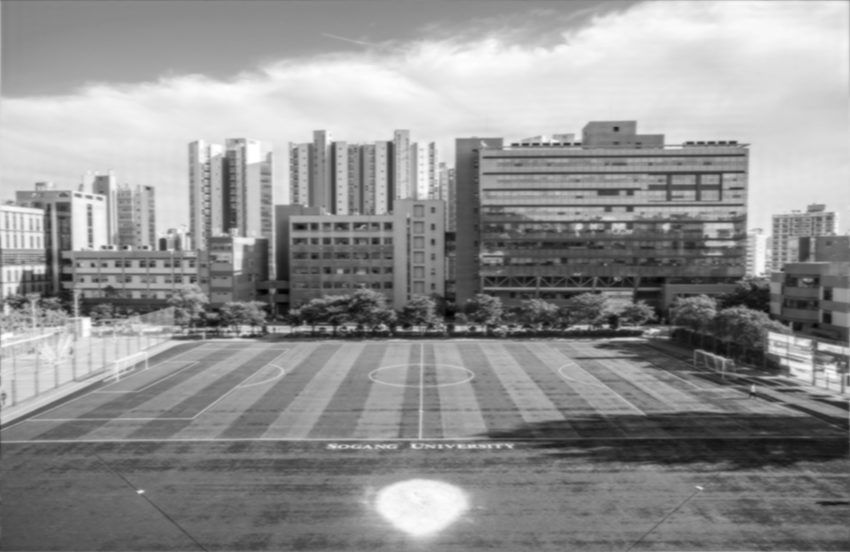
\includegraphics[scale=0.15]{../data/sogang_0p00025_undegraded.png}
}
\subfigure[\textbf{Weiner, $k=0.00025$, 35.07 dB}]{
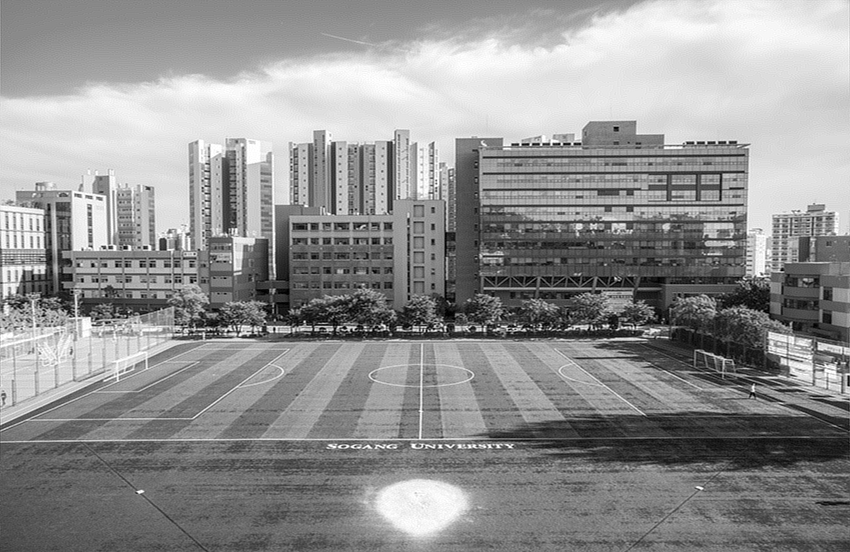
\includegraphics[scale=0.15]{../data/sogang_wienerp00025_undegraded.png}
}
\subfigure[Degraded, $k=0.001$, 22.08 dB]{
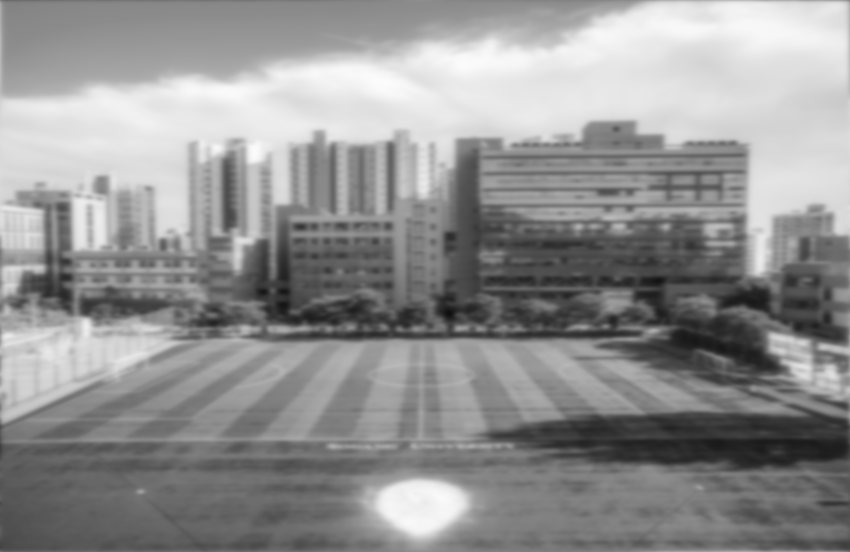
\includegraphics[scale=0.15]{../data/sogang_0p001_degraded.png}
}
\subfigure[Inverse, $k=0.001$, 22.60 dB]{
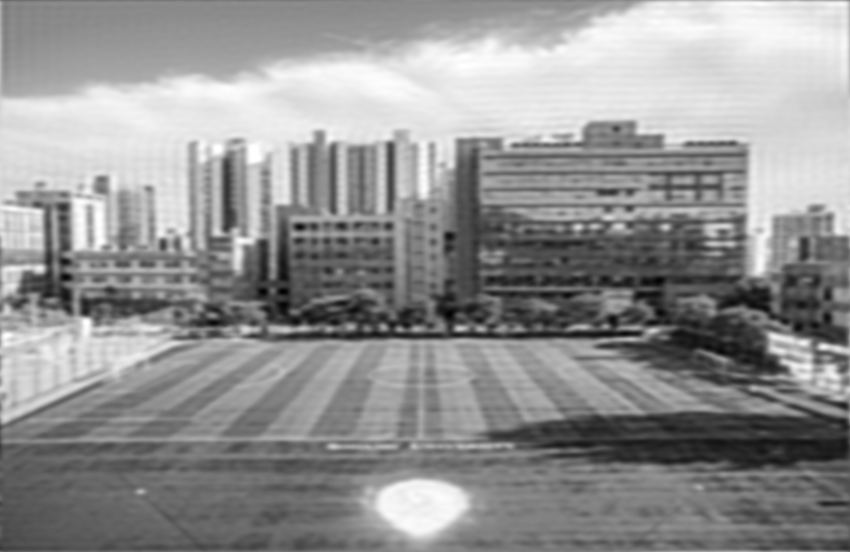
\includegraphics[scale=0.15]{../data/sogang_0p001_undegraded.png}
}
\subfigure[Weiner, $k=0.001$, 25.33 dB]{
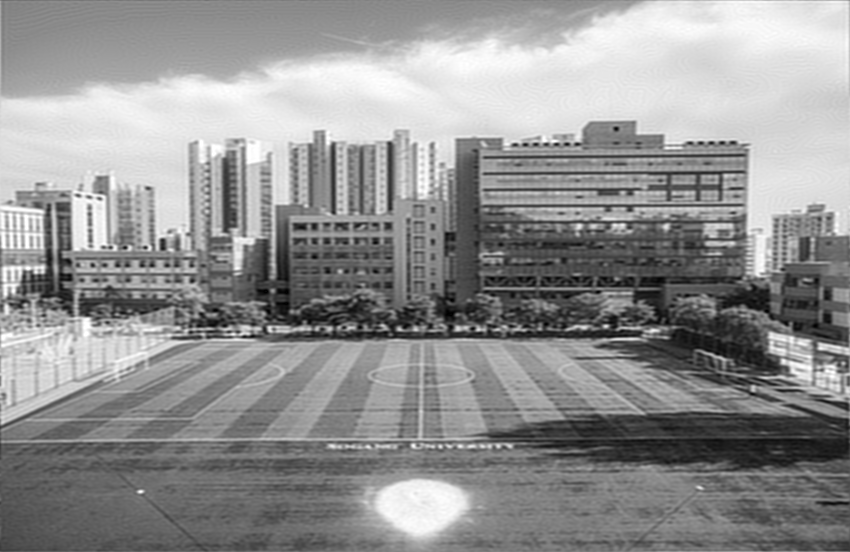
\includegraphics[scale=0.15]{../data/sogang_wienerp001_undegraded.png}
}
\subfigure[Degraded, $k=0.0025$, 20.67 dB]{
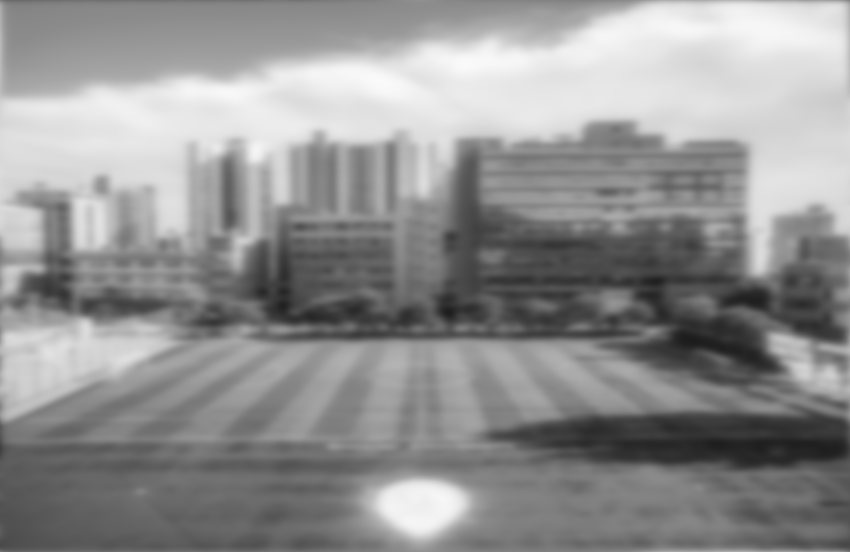
\includegraphics[scale=0.15]{../data/sogang_0p0025_degraded.png}
}
\subfigure[Inverse, $k=0.0025$, 21.92 dB]{
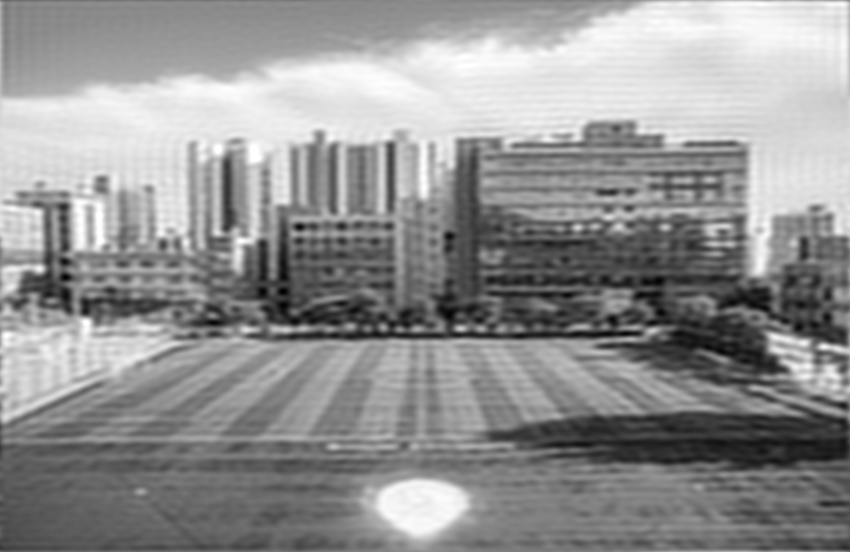
\includegraphics[scale=0.15]{../data/sogang_0p0025_undegraded.png}
}
\subfigure[Weiner, $k=0.0025$, 22.71 dB]{
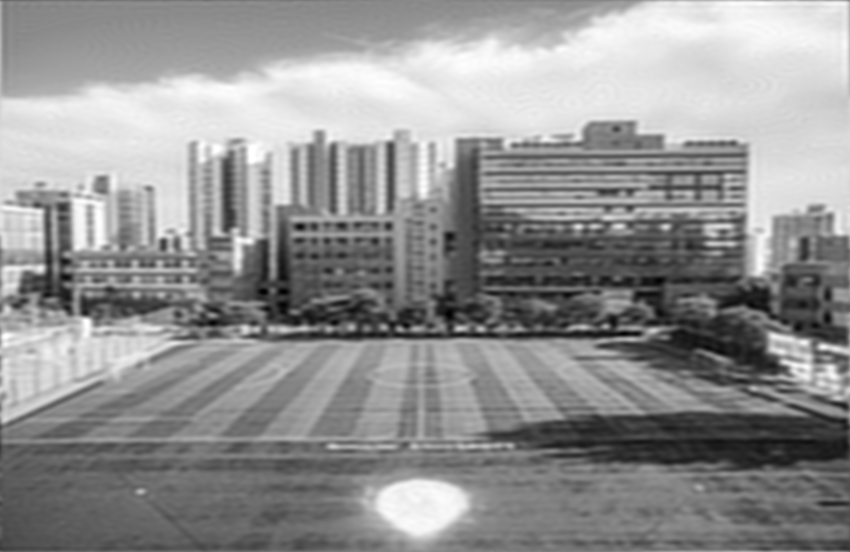
\includegraphics[scale=0.15]{../data/sogang_wienerp0025_undegraded.png}
}
\caption{복원을 적용한 결과물 영상들.}\label{fig:recon}
\end{figure}

복원이 적용된 영상들을 inverse fourier transform 을 통해 spatial domain 으로 가져온 모습을 Fig.~\ref{fig:recon} 에서 볼 수 있다. 전체적으로 Weiner filter 가 복원 성능이 단순한 inverse filtering 에 비해서 뛰어나다. 특히 $k=0.00025$ 인 경우에는 10dB 가까이 복원 성능이 향상됐다. 이 때 Weiner filter 를 거친 결과물은 PSNR 이 35.07dB로, 육안으로 봤을 때 원본 영상과 거이 차이가 없엇다. degradation 이 심하게 된 $k=0.0025$ 의 경우에는 inverse filter 와 Weiner filter 모두 복원이 큰 효과를 발휘하지 못했다.

\vspace{0.1in}
\noindent\textbf{검토사항:} 이전에 degradation 을 \eqref{eq:degrad}, \eqref{eq:cplx_degrad} 와 같이 표현을 했었다. Inverse filtering 을 사용하는 경우에는 복원이 \eqref{eq:filtered} 와 같이 표현이 될 수 있다.

\begin{align}
  \hat{F(u, v)} &= \frac{1}{H(u, v)}G(u, v) \\
                &= \frac{1}{H(u, v)}(F(u, v)H(u, v) + N(u, v)) \\
                &= F(u, v) + \frac{N(u, v)}{H(u, v)} \label{eq:filtered}
\end{align}

문제는 $H(u, v) \approx 0$ 인 경우에는 $\frac{N(u, v)}{H(u, v)}$ 이 발산하면서 $F(u, v)$ 를 압도해버리게 된다. 특히 이번 과에서 사용한 exponential 모델의 경우에는 $H$ 가 매우 빠르게 0 으로 수렴한다. 또한 8비트로 quantization 된 영상을 사용했기 때문에 noise 를 추가로 가하지 않아도 최대 $1/255$ 크기의 노이즈가 존재한다. 이 때문에 inverse filtering 을 사용하는 경우에는 복원 영역을 $r$ 을 이용해서 지정하고, Weiner filter 에서는 $\frac{S_n(u, v)}{S_s(u, v)}$ 상수를 지정해준다 (물론 실제로는 영상에 따라서는 quantization 노이즈의 실제 level이 1/255 보다 작을 수 있다). 결국 quantization noise 와 같이 자연적으로 영상에 존재하는 noise 성분으로 인해서 deconvolution 기반 방법을 통한 영상의 완벽한 복원은 가능하지 않다. 추가로, 컴퓨터를 통해서 연산을 수행하는 경우에 IEEE-754 실수 표현방법을 사용하게 되는데, 이 실수는 표현 가능한 유효 숫자와 실수 범위가 제한적이기 때문에 $H(u, v)$ 가 작아질수록 오차가 누적되게 된다. $1/H(u, v)$ 를 계산하게 되는 경우 특히 오차의 영향이 커진다.


\section{conclusion}
이번 과제에서는 2D convolution 을 이용한 linear spatial filtering 을 C++ 로 구현하였고, gaussian blur, box blur, laplacian edge enhancement, sobel edge detection 등의 고전적인 image operation 들을 직접 수행하였다. 이들의 효과를 실제 영상에 적용하여 확인하였고, extension padding 과 zero padding 두 종의 padding 을 구현하여 이들의 차이 또한 분석하였다.

\end{document}

\end{table}
